\chapter{Example Dataset}
\label{cha:exampleDataset}

In this chapter, we delve into the structure of the dataset on an example to simplify its extraction and usage later in this work. We will primarily focus on the data the Apple Watch can provide, highlighting key metrics such as heart rate, distance, step count and other relevant physiological and activity parameters. This includes showcasing the various types of information the Apple Watch tracks and identifying which pieces of information are crucial for this work.

\section{Structure of the Dataset}

The dataset consists of recorded Apple Watch values. A total of two people of each sex were wearing the smartwatch over a period of two years. During this time, a wide variety of values were collected. Initially, the data were exported in Extensible Markup Language (XML) format and were converted into Comma-Separated Values (CSV) tables using the implemented program to simplify data usage. 

CSV files are often preferred over XML for data handling in Python due to their simplicity, readability, and performance. CSV files consist of plain text, making them easy to read and parse, whereas XML files have a more complex structure with nested tags. Parsing CSV files is faster and more efficient, especially for large datasets, thanks to Python's robust libraries like 'pandas' and the built-in 'csv' module. These libraries provide convenient functions for handling CSV data.

Our converted CSV table consists of 38 columns, but this study primarily used only the columns 'type', 'value', 'unit', 'startDate' and 'endDate', so five columns in total and all measured data categories are already listed in the 'type' column.

We are not using any other columns, because the other columns were mostly not measured correctly or not measured at all and therefore did not provide sufficient data. 

The 'type' column refers to the type of recording, for example, whether the watch recorded a running session, the calories burned, or the person's heart rate. The 'value' column stores all measured values, and the 'unit' column represents the corresponding unit, such as minutes, kilometers, calories, etc. The 'startDate' and 'endDate' columns are particularly important for determining the exact interval of the recording.

\section{Heart Rate, Energy Burned and Walked Distance Analysis}

We started by filtering all entries in the 'type' column of the CSV table labeled 'HeartRate,' with a particular focus on the 'value' 32.

\subsection{Daily Behavior and Correlations in the Example Dataset}
We selected the day with the highest heart rate and filtered all the data from that day, such as heart rate, calories burned and distance traveled, to see how the high heart rate relates to other features. This resulted in the following graphs for two healthy individuals:

\FloatBarrier
\begin{figure}[h!]
  \centering
  \begin{minipage}[b]{0.8\linewidth}
    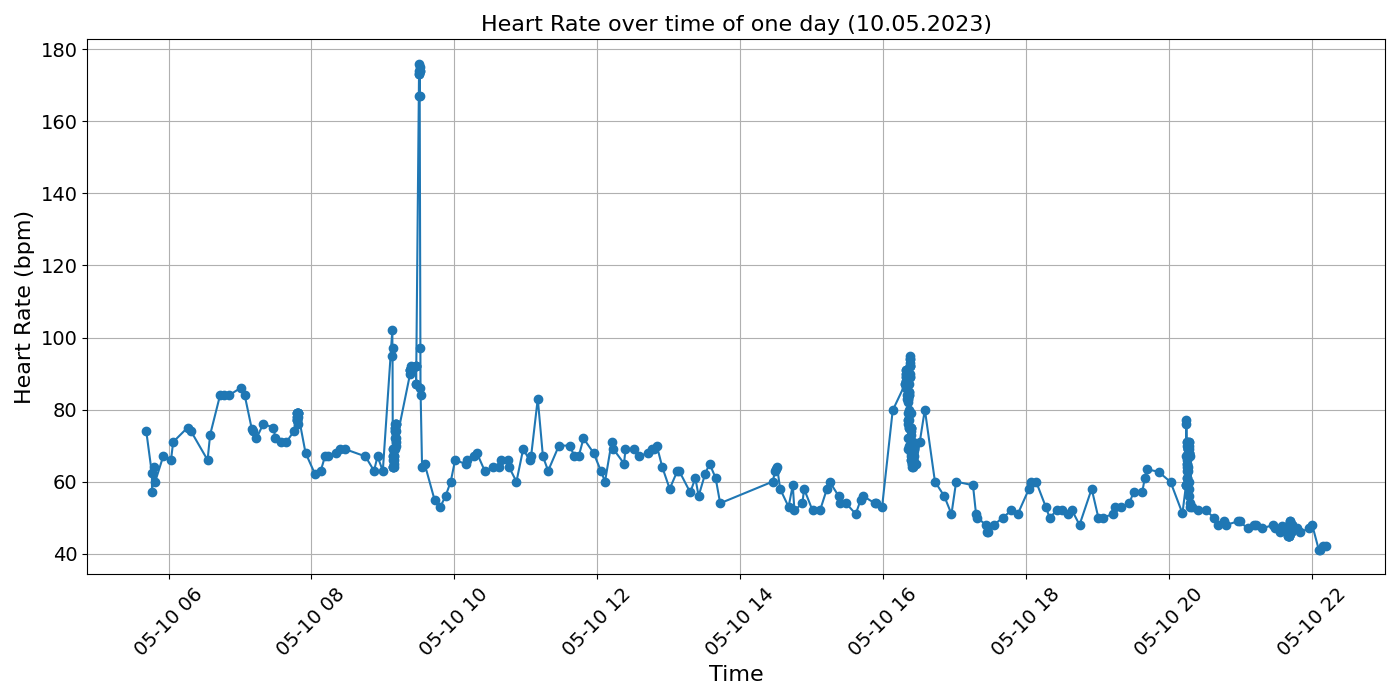
\includegraphics[width=\linewidth]{Master Thesis/Plots/HeartRate1day_Michi.png}
    \caption{Day of maximal heart rate in a male subject over 30 years of age}
    \label{fig:MaxHeartMichi}
  \end{minipage}
  \quad % Fügt etwas Platz zwischen den Bildern ein
  \begin{minipage}[b]{0.8\linewidth}
    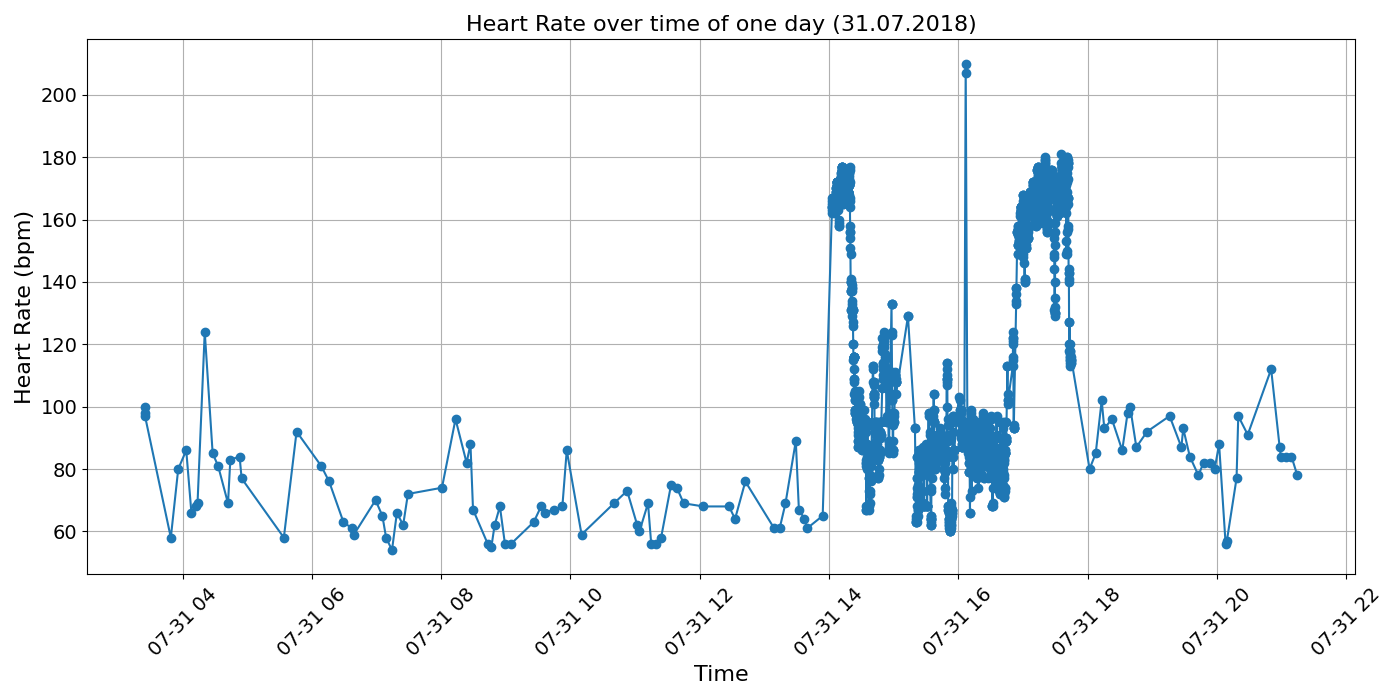
\includegraphics[width=\linewidth]{Master Thesis/Plots/HeartRate1day_Tanja.png}
    \caption{Day of maximal heart rate in a female test subject under 25 years of age}
    \label{fig:MaxHeartTanja}
  \end{minipage}
\end{figure}
\FloatBarrier

The provided figures ~\ref{fig:MaxHeartMichi} and ~\ref{fig:MaxHeartTanja} show heart rate data over the course of one day for two subjects. The first plot represents the heart rate of a subject over 30 years of age on May 10, 2023. The second plot illustrates the heart rate of a subject on July 31, 2018.

The young female subject exhibits significant variations in heart rate throughout the day, with notable peaks between 2 PM and 6 PM reaching up to 201 bpm, and a minimum of 54 beats per minute (bpm). The subject in the 30 to 35 years age range shows a more stable heart rate pattern, with a maximum of 176 bpm and a minimum of 41 bpm.

So far, the analysis of the dataset focused solely on heart rate. It becomes particularly interesting when we include additional factors in our examination. For this reason, we chose the types 'BasalEnergyBurned', 'ActiveEnergyBurned', and 'HeartRate'. The feature 'BasalEnergyBurned' refers to a type of sampling that measures the time the user has spent on activities during the specified day, including whole-body movements ~\cite{appleBasalEnergyBurnedApple}.
The feature 'ActiveEnergyBurned' is the energy the user burned due to physical activity and movement. These samples should not include the resting energy burned during the sample duration ~\cite{appleActiveEnergyBurnedApple} and 'HeartRate' is the pulse measurement ~\cite{appleHeartRateApple}. After selecting the types, the focus was again on the day with the highest bpm value.

\FloatBarrier
\begin{figure}[h!]
  \centering
    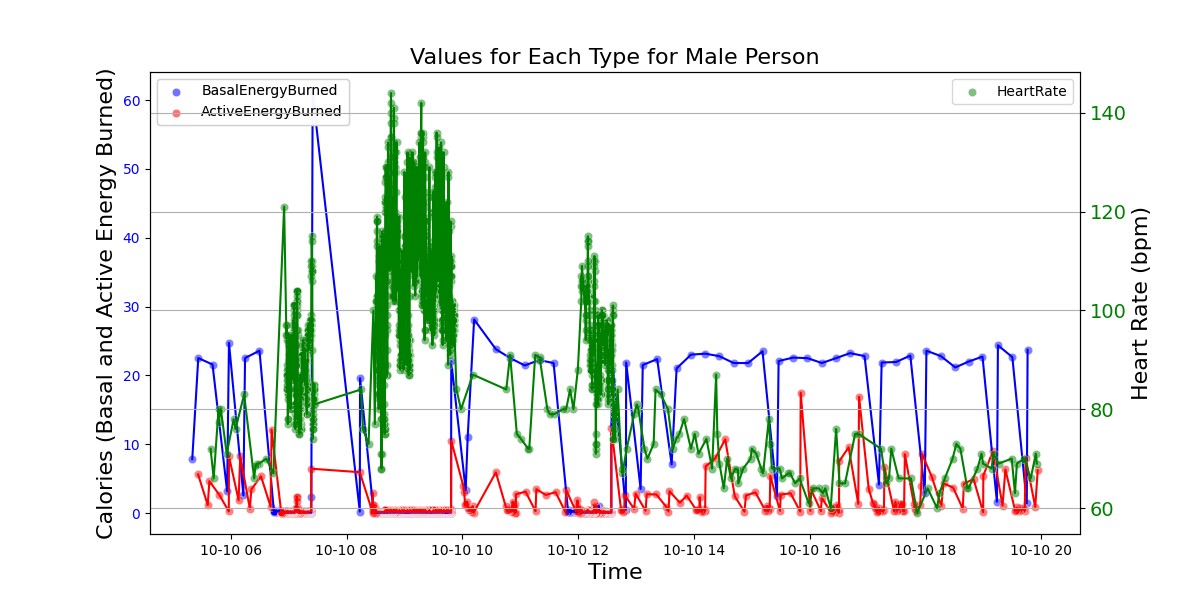
\includegraphics[width=1.0\textwidth]{Master Thesis/Plots/Values_Mean_Male.png}
    \caption{Day of maximal heart rate in a male subject over 30 years of age all relevant values}
    \label{fig:ValuesMale}
    \end{figure}
\FloatBarrier

\FloatBarrier
\begin{figure}[h!]
  \centering
    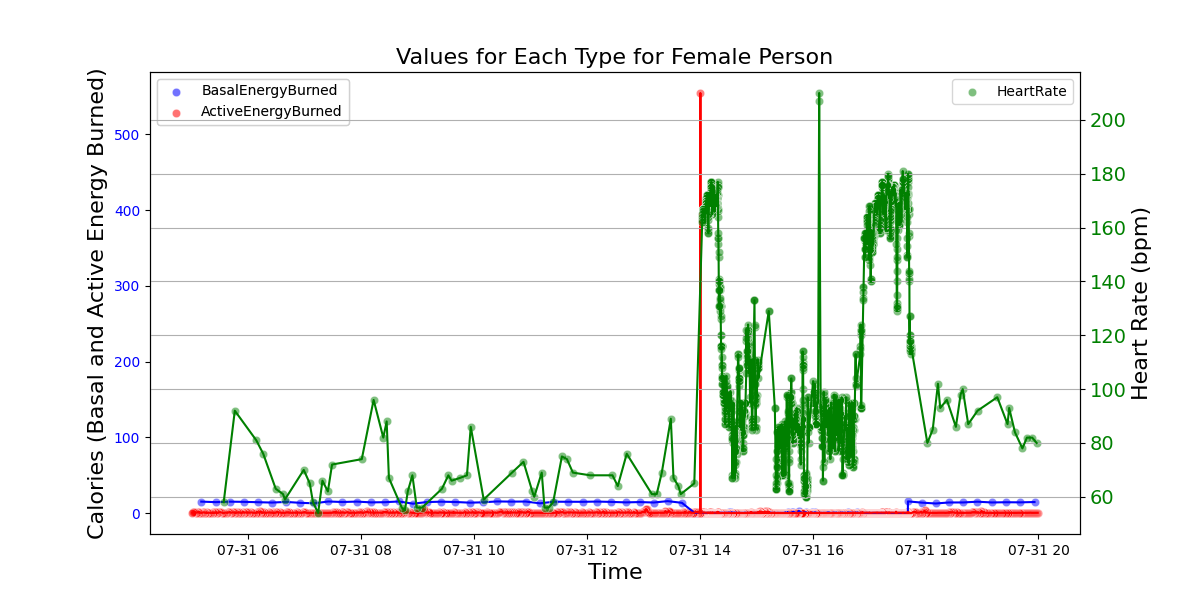
\includegraphics[width=1.0\textwidth]{Master Thesis/Plots/Values_Mean_Female.png}
    \caption{Day of maximal heart rate in a female test subject under 25 years of age all relevant values}
    \label{fig:ValuesFemale}
\end{figure}
\FloatBarrier

The key observations of figure ~\ref{fig:ValuesMale} and figure ~\ref{fig:ValuesFemale} are that the older male subject shows less variation in heart rate and energy burned, possibly indicating a more sedentary lifestyle or a more controlled and steady day of activities.
The younger female subject exhibits extreme heart rate values that are likely to be because of extreme stress or physical activity.
The relationship between heart rate and energy burned is not directly apparent in these plots, suggesting that individual physical responses and activities may vary widely.
In both plots, the exact times of day when heart rate and energy expenditure peak could be further analyzed to understand the subjects activity patterns and potential health implications, but we will leave that at this point of the work.

\subsection{Weekly Behavior and Correlations in the Example Dataset}

At this stage of the thesis, only the day with the highest bpm value has been taken into consideration. In order to be able to make better statements and analyze abnormalities, we want to look at a whole week of the test subjects. As the plots for this are very difficult to read and analyze, the days of the week 25.07 to 31.07 were added together and the average of these days was then calculated. 
It should also be mentioned that we did not consider the steps but the distance covered by the test subjects as we do not know the exact step size. 
The results can be seen in the following table: 

\FloatBarrier
\begin{table}[h!]
\centering
\begin{tabular}{|l|c|r|}
\hline
\textbf{feature} & \textbf{female 20 - 25 years } & \textbf{male  30 - 35 years} \\ \hline
avg. heart rate      & 99.89 bpm         &  76.89 bpm       \\ \hline
avg. active energy burned      & 1620.24 kcal         & 836.19 kcal       \\ \hline
avg. basal energy burned & 1362.89 kcal         & 2045.07 kcal      \\ \hline
avg. distance walking running      & 18.54 km         & 15.67 km     \\ \hline
\end{tabular}
\caption{Table of important characteristics with the average value in a particular week}
\label{table:example}
\end{table}
\FloatBarrier

It is now noticeable again that the female test subject has a higher pulse rate on average than the male test subject. Besides, this is probably mainly due to the age category. One discrepancy that is particularly noticeable is, that the female test subject has a significantly higher average calorie consumption in relation to actively consumed calories. Although, their basal energy burned value is almost the same. This value is very different for the male test subject. On the other hand, we see a higher value for the average kilometers covered per day this week for the male subject, but both exceed the recommended daily distance of 8 km. This is generally a satisfactory result.

\subsection{Exploring the Example Dataset with Cross Entropy}

Initially, the focus of the study was on heart rate, as this, along with calories burned, is most commonly recorded.
But how do we manage to compare the two sex and their distributions effectively without just relying on our eyes? 

To gain a detailed understanding of the heart rate and its measurement, all available values were first illustrated in a graph.
This is where cross-entropy comes into play. In the following, this methodology was applied to the four features.

\FloatBarrier
\begin{figure}[h!]
  \centering
  \begin{subfigure}{.55\textwidth}
    \centering
    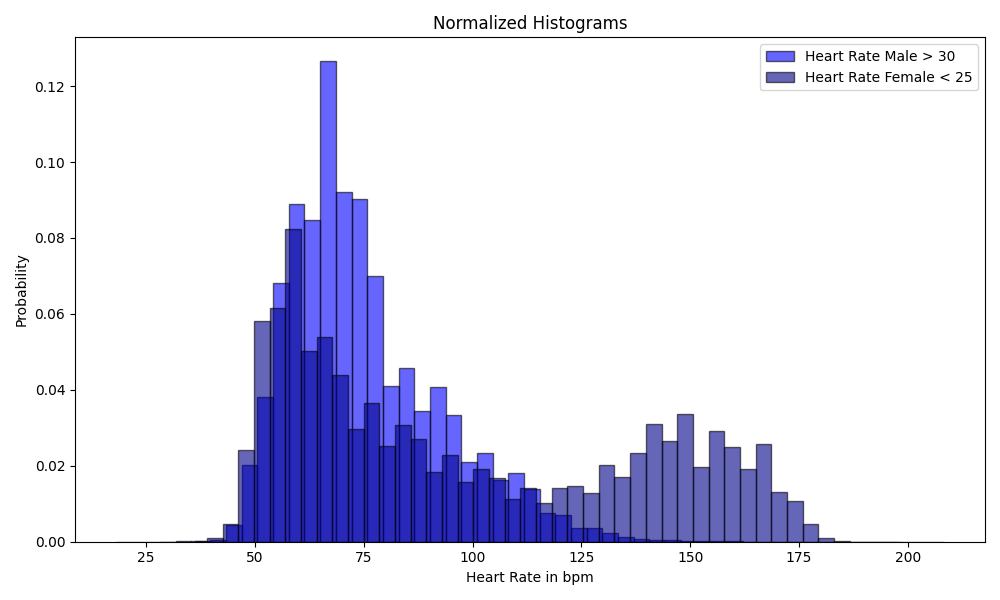
\includegraphics[width=.8\linewidth]{Master Thesis/Plots/CrossEntro_HeartRate.png}
    \caption{Distributions of heart rates of male and female subject}
    \label{fig:heart_rate}
  \end{subfigure}%
  \begin{subfigure}{.55\textwidth}
    \centering
    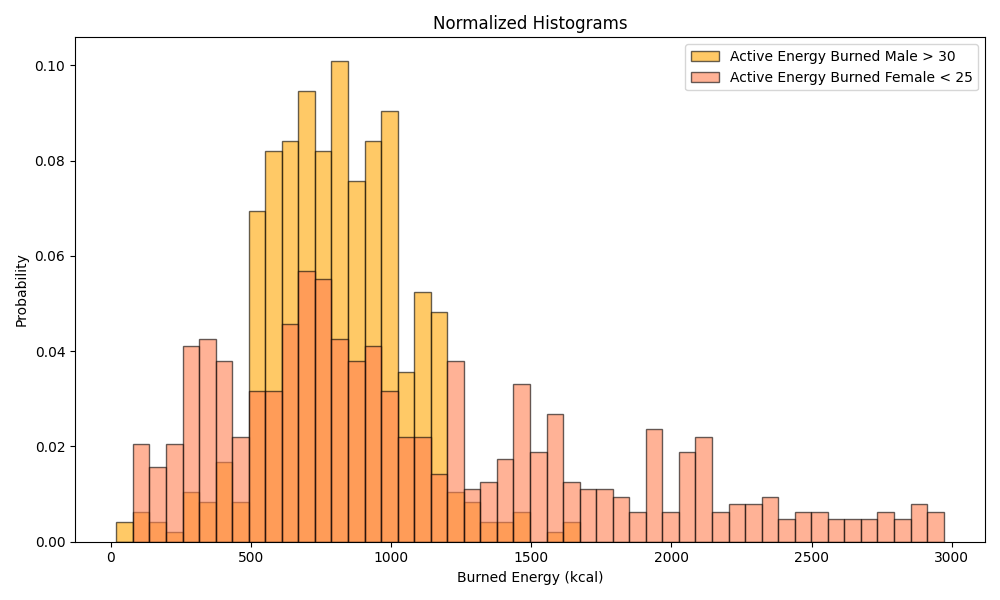
\includegraphics[width=.8\linewidth]{Master Thesis/Plots/CrossEntro_ActiveEnergyBurned.png}
    \caption{Distributions of active energy burned of male and female subject}
    \label{fig:active_energy}
  \end{subfigure}
  \newline
  \begin{subfigure}{.55\textwidth}
    \centering
    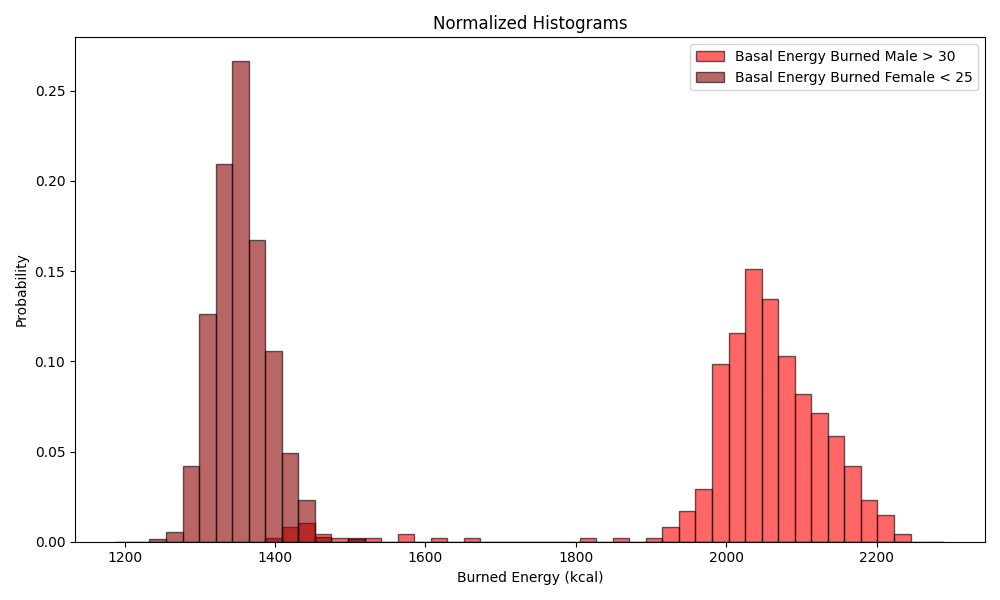
\includegraphics[width=.8\linewidth]{Master Thesis/Plots/CrossEntro_BasalEnergyBurned.png}
    \caption{Distributions of basal energy burned of male and female subject}
    \label{fig:basal_energy}
  \end{subfigure}%
  \begin{subfigure}{.55\textwidth}
    \centering
    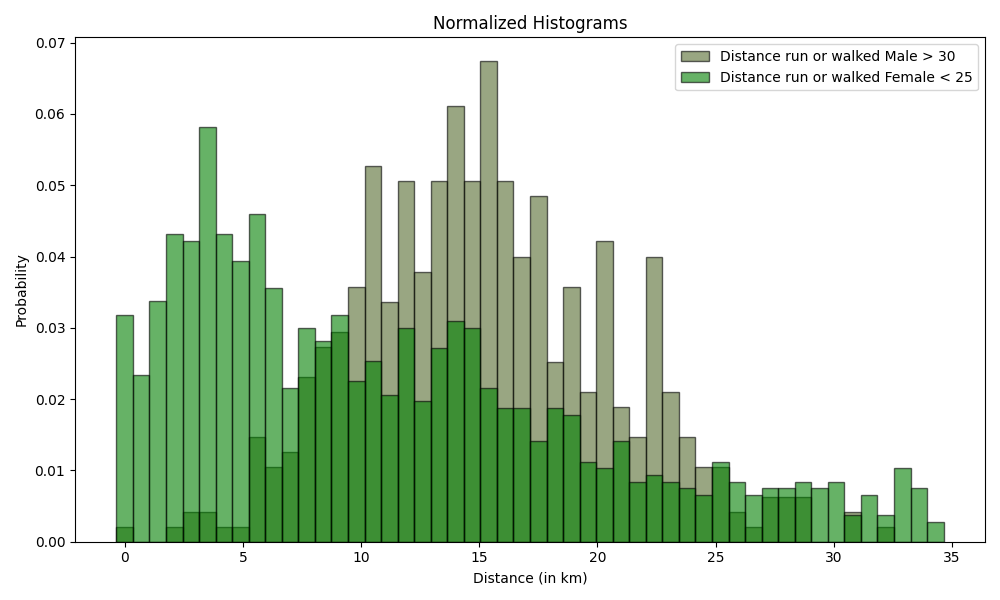
\includegraphics[width=.8\linewidth]{Master Thesis/Plots/CrossEntro_Distance.png}
    \caption{Distributions of walked or jogged distances of male and female subject}
    \label{fig:distance}
  \end{subfigure}
  \caption{Distributions for different data types of the example dataset}
  \label{fig:cross_entropy}
\end{figure}
\FloatBarrier

The presented plots in ~\ref{fig:cross_entropy} illustrate the distributions of various measurements for male and female subjects. The histograms depict how heart rate, active energy burned, basal energy burned, and walked or jogged distances differ between the two subjects.

In the first plot ~\ref{fig:heart_rate}, the distributions of heart rates for male and female subjects are shown. The plot reveals that the heart rates of female subjects (in blue) are generally higher than those of male subjects (in lighter blue). Notably, the heart rate distribution of female subjects is concentrated between 60 and 90 bpm (beats per minute).

The second plot ~\ref{fig:active_energy} displays the distributions of active energy burned for male and female subjects. The distribution for male subjects (yellow) tends to be higher than that for female subjects (orange). This may indicate that male subjects engaged in more intensive physical activities during the tests.

The third plot ~\ref{fig:basal_energy} represents the distributions of basal energy burned for male and female subjects. Again, a clear distinction between sex is observed. The distribution for female subjects (dark red) is generally lower than that for male subjects (red), which may reflect differences in basal metabolic rate and metabolism.

The fourth plot ~\ref{fig:distance} shows the distributions of walked or jogged distances for male and female subjects. It is evident that female subjects (green) generally covered shorter distances compared to male subjects (dark green). This could indicate differences in physical activity levels and endurance.

\newpage

Overall, it is clear that none of the distributions are identical. To quantify this more precisely, the cross-entropy value was calculated, as described in chapter ~\ref{cha:methods}. 

The best results were obtained for 'ActiveEnergyBurned' at 3.48, 'HeartRate' at 3.57, and 'DistanceWalkingRunning' at 3.95. These values suggest that these distributions are the most similar, although they are still far from 1, which would indicate an ideally identical or nearly identical distribution. For 'BasalEnergyBurned' at 33.70, the worst result was obtained, and a quick glance shows that these distributions are completely different.

